\section{TINJAUAN PUSTAKA}

% Ubah konten-konten berikut sesuai dengan isi dari tinjauan pustaka
\subsection{Hasil penelitian terdahulu}
\subsubsection{Rancang Bangun Anemometer Ultrasonik dalam Ruangan}

Penelitian yang dilakukan oleh Ahmad Harris Abdillah dengan judul 'Rancang Bangun Anemometer 
Ultrasonik dalam Ruangan' \parencite{Abdillah2022}. Penelitian ini menggunakan Arduino Uno sebagai mikrokontroler
dan sensor HCS04 sebagai sensor ultrasonicnya. Namun hasil pengukuran yang diperoleh
masih memiliki error yang cukup besar yaitu maksimal 11,11 persen dan minimal sebesar 0,66 persen

\begin{figure}[h!]
	\centering
	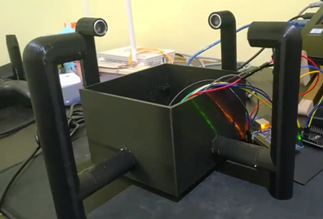
\includegraphics[width=0.5\linewidth]{gambar/fig_anemometer_abdillah_prototipe}
	\caption{Rancang Bangun Anemometer Ultrasonic \parencite{Abdillah2022}}
	\label{abdillah_anemo_prototipe}
\end{figure}

\subsubsection{Rancang Bangun \emph{Thermal-Based Anemometer} dan Arah Angin untuk Aliran Udara Rendah}

Penelitian yang dilakukan oleh Radiktya Dewanto Cahyolaksono dengan judul 'Rancang Bangun \emph{Thermal-Based Anemometer} dan Arah Angin untuk 
Aliran Udara Rendah' \parencites{Cahyolaksono2022}. Proses pengukuran kecepatan angin menggunakan prinsip perpindahan panas. Anemometer Thermal-Based
ini dapat digunakan didalam ruangan dan mampu mengukur kecepatan angin terendah sebesar 0,60 m/s dan kecepatan angin
tertinggi sebesar 5,10 m/s dengan arah angin dinotasikan dalam derajat (theta).

\begin{figure}[h!]
	\centering
	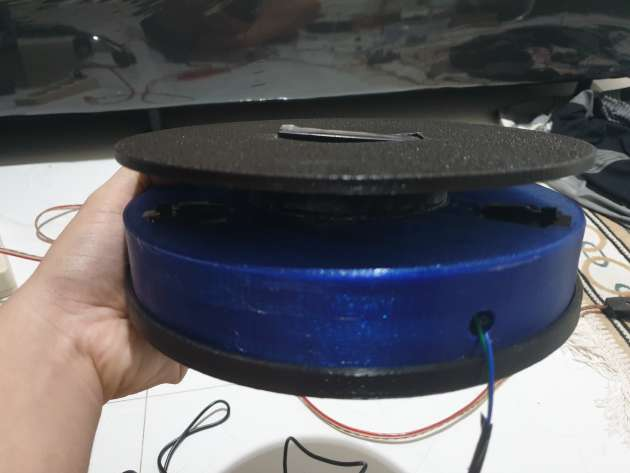
\includegraphics[width=0.5\linewidth]{gambar/fig_alat_cahyolaksono}
	\caption{Rancang Bangun Thermal-Based Anemometer \parencite{Cahyolaksono2022}}
	\label{fig:figalatcahyolaksono}
\end{figure}

\subsection{Angin}

% Contoh penggunaan referensi dari pustaka
Angin adalah udara yang bergerak dari daerah yang bertekanan udara tinggi (maksimum) ke daerah yang bertekanan udara rendah (minimum) yang disebabkan oleh
pemanasan yang tidak merata oleh sinar matahari \parencites{turgeon2022wind}. Angin tidak 
dapat dilihat secara kasat mata namun dapat dirasakan gayanya. Keberadaan angin dapat dibuktikan dengan melihat daun-daun yang berterbangan ataupun melihat bendera yang berkibar. Selain 
itu, angin sudah dimanfaatkan sejak dahulu kala untuk membantu manusia mengeringkan pakaian dan 
berlayar di laut lepas.

Tekanan udara merupakan salah satu parameter pembentuk arah dan kecepatan angin.
Suatu tenaga yang bekerja untuk menggerakkan massa udara dalam 
setiap satuan luas tertentu dan menekan arah pergerakan massa udara tersebut searah 
gaya gravitasi bumi disebut tekanan udara \parencites{yulkifli2016pengukuran}. Satuan tekanan udara adalah milibar (mb) atau Hecto Pascal (hPa). 
Tekanan udara dipengaruhi oleh temperatur/suhu udara yang terjadi pada suatu tempat dan 
waktu, apabila temperatur udara tinggi maka volume molekul/partikel udara akan berkembang 
sehingga tekanan udara menjadi rendah dan berbanding sebaliknya. 

\subsection{Kecepatan Angin}


Kecepatan Angin merupakan kecepatan horizontal yang dapat teukur pada ketinggian 2 meter dari tanah yang ditanami rumput /parencites{Abdillah2022}.
Hal ini untuk memperjelas bahwa kecepatan angin dapat dipengaruhi oleh karakteristik permukaan yang dilaluinya.
Selain itu, kecepatan angin juga dipengaruhi perbedaan tekanan udara antara tempat
asal dan tujuan angin (sebagian faktor pendorong) dan resistensi medan yang dilaluinya. Apabila tekanan udara tempat asal lebih tinggi dan tidak
ada medan resistansi yang menghalangi laju kecepatan angin maka kecepatan angin dapat dikatakan cukup tinggi.

Terdapat skala untuk mengukur kecepatan angin yang dinamakan Beafourt Scale (Skala Beaufort) /parencites{Cahyolaksono2022}. 
Beafourt Scale adalah ukuran empiris yang berkaitan dengan kecepatan angin untuk pengamatan kondisi di darat atau di laut. Skala ini ditemukan oleh
Francis Beaufort pada tahun 1805. Beaufort mengukur kecepatan angin dengan menggambarkan pengaruhnya pada kecepatan kapal dan gelombang air laut \parencite{book2002wind}. 
Skala
Beaufort menggunakan angka dan simbol. Semakin besar angka skala Beaufort, maka
semakin kencang angin berhembus dan bahkan bisa semakin merusak. Skala Beaufort
dimulai dari angka 0 untuk hembusan angin yang paling tenang sampai angka 12 untuk
hembusan angin yang dapat menyebabkan kehancuran. Skala Beaufort masih digunakan
sampai sekarang untuk memperkirakan kecepatan angin.

\begin{table}[h!]
	\label{tbl:beaufortScale}
	\centering
	\caption{Skala Beaufort \parencite{Abdillah2022}}
	\begin{tabular}{|c|c|c|p{4cm}|}
		\hline
		\rowcolor{lightgray}
		Beaufort Number  & Description of Wind & Speed (m/s) & Description of Wind Effects \\
		\hline
		0 & Calm & Less than 0.4 & No noticeable wind \\
		\hline
		1 & Light Airs & 0.4 - 1.5 & No noticeable wind \\
		\hline
		2 & Light Breeze & 1.6 - 3.3 & Wind felt on face \\
		\hline
		3 & Gentle Breeze & 3.4 - 5.4 & Wind extends light
		flag, Hair is
		disturbed, Clothing
		flaps \\
		\hline
		4 & Moderate Breeze & 5.5 - 7.9 & Wind raises dust,
		dry soil, and loose
		paper, Hair
		disarranged \\
		\hline
		5 & Fresh Breeze & 8.0 - 10.7 & Force of wind felt
		on body, Drifting
		snow becomes
		airborne, Limit of
		agreeable wind on
		land \\
		\hline
		6 & Strong Breeze & 10.8 - 13.8 & Umbrellas used
		with difficulty, Hair
		blown straight,
		Difficulty to walk
		steadily, Wind
		noise on ears
		unpleasant,
		Windborne snow
		above head height
		(blizzard) \\
		\hline
		7 & Moderate Gale & 13.9 - 17.1 & Inconvenience felt
		when walking \\
		\hline
		8 & Fresh Gale & 17.2 - 20.7 & Generally impedes
		progress, Great
		difficulty with
		balance in gusts \\
		\hline
		9 & Strong Gale & 20.8 - 24.4 & People blown over
		by gusts \\
		\hline
	\end{tabular}
\end{table}
	
\subsection{Anemometer}

Anemometer merupakan sebuah perangkat untuk mengukur  kecepatan angin. Alat ini sering 
digunakan oleh Badan Meterologi Klimatologi dan Geofisika (BMKG) untuk memprediksi cuaca. Nama anemometer berasal dari Bahasa Yunani \textit{anemos} yang berarti angin. Anemometer ini pertama kali diperkenalkan 
oleh Leon Batista Alberti dari italia pada tahun 1450. Pada saat itu, model anemometer pertama menggunakan mekanisme sederhana yang terdiri dari sebuah disk 
yang ditempatkan tegak lurus terhadap angin. Angin akan menggerakkan bendera dan menghasilkan sudut kemiringan disk kekuatan angin sesaat. 

\begin{figure}[h!]
	\centering
	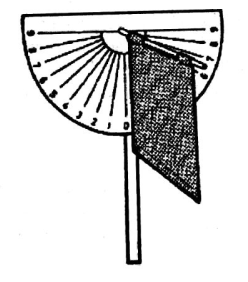
\includegraphics[width=0.3\linewidth]{gambar/anemometerGen1}
	\caption{Anemometer Generasi Pertama \parencite{Panjaitan2018}}
	\label{fig:anemometergen1}
\end{figure}

Secara umum ada dua jenis anemometer, yaitu anemometer yang mengukur kecepatan angin (\textit{
velocity anemometer}) dan anemometer yang mengukur tekanan angin (\textit{pressure anemometer}).
Salah satu jenis anemometer adalah ultrasonic anemometer yang memanfaatkan suara sonic dengan frekuensi tinggi dan mengukur \textit{Time of Flight (ToF)} yang kemudian diubah menjadi kecepatan angin.

\subsubsection{Cup Anemometer}

\begin{figure}[h!]
	\centering
	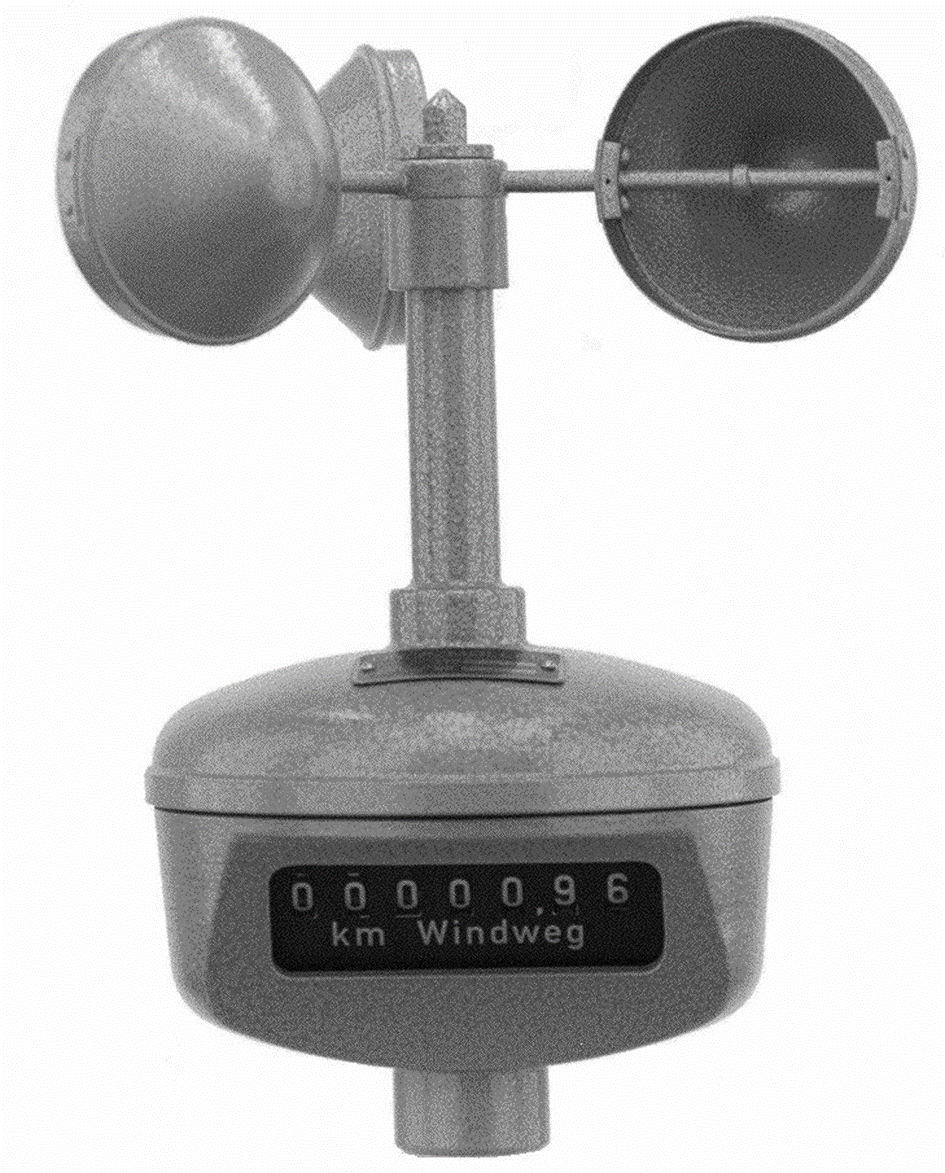
\includegraphics[width=0.3\linewidth]{gambar/anemometerCup}
	\caption{Cup Anemometer \parencite{figCupAnemometer}}
	\label{fig:anemometercup}
\end{figure}

Diciptakan oleh Dr. John Thomas Romney Robinson dari Armargh Observatory pada tahun 1846.
Cup Anemometer adalah velocity anemometer yang mempunyai baling-baling berbentuk setengah lingkaran dan menyerupai mangkok kecil. Ketika tertiup angin, mangkok 
yang terdapat pada anemometer akan bergerak sesuai arah angin. Makin besar kecepatan angin meniup mangkok tersebut, makin cepat pula kecepatan 
berputarnya piringan mangkok tersebut, makin cepat pula kecepatan berputarnya piringan mangkok. Dari jumlah putaran dalam satu detik maka dapat 
diketahui kecepatananginnya. Didalam anemometer terdapat alat pencacah yang akan menghitung kecepatan angin.

\subsubsection{Windmill Anemometer}

\begin{figure}[h!]
	\centering
	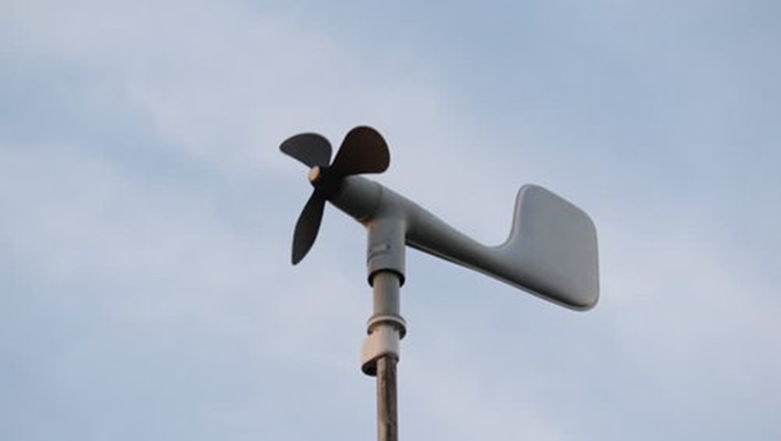
\includegraphics[width=0.3\linewidth]{gambar/anemometerWindmill}
	\caption{Windmill Anemometer}
	\label{fig:anemometerwindmill}
\end{figure}


Windmill Anemometer adalah velocity anemometer di mana kincir angin didorong oleh aliran udara, dan rotasi ditransmisikan melalui gearing ke dial atau 
mekanisme perekaman lainnya. Dalam beberapa instrumen, baling-baling dan dial yang berputar berada pada bidang yang sama yaitu, keduanya vertikal, 
sementara di lain dial adalah horizontal. Dalam jenis kincir angin, pengoperasian pengukuran udara melibatkan pembacaan dial pada awal dan akhir 
periode yang diukur. Instrumen kincir angin dapat dilengkapi dengan pegangan ekstensi, menyediakan bentuk kendali jarak jauh; digunakan untuk mengukur 
kecepatan udara di tempat yang tidak dapat diakses.

\subsubsection{Hot Wire/Thermal Anemometer}

Thermal Anemometer atau dikenal juga dengan Hot Wire Anemometer adalah velocity anemometer menggunakan kawat yang sangat halus dan dipanaskan. Udara yang mengalir
melewati kawat akan mendinginkan kawat. Terdapat dua mode operasi yang dimungkinkan; dalam satu kasus dengan
mengukur daya yang dibutuhkan untuk menjaga sensor pada suhu konstan, atau, di sisi
lain, dengan mengukur suhu sensor dengan pasokan daya yang konstan.

\begin{figure}[h!]
	\centering
	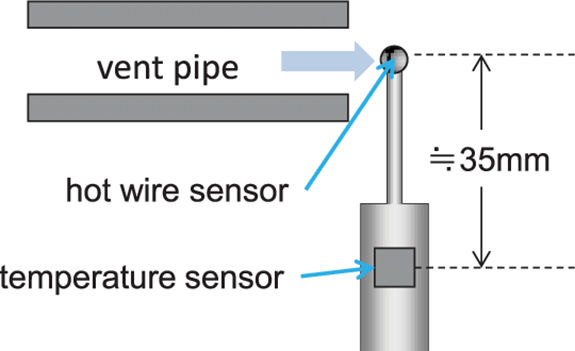
\includegraphics[width=0.4\linewidth]{gambar/anemometerHotWire}
	\caption{Hot-Wire Anemometer}
	\label{fig:anemometerhotwire}
\end{figure}


\subsubsection{Ultrasonic Anemometer}

Pertama kali diperkenalkan pada tahun 1950, ultrasonic anemometer adalah velocity anemometer yang menggunakan gelombang suara ultrasonik 
untuk mengukur kecepatan angin. Dengan memanfaatkan Time of flight pulsa suara yang merambat di udara antara pasangan transduser menyediakan metode lebih lanjut untuk mengukur kecepatan angin. 
Karena responnya yang cepat, anemometer ultrasonik sangat 
cocok untuk pengukuran lapangan fluktuasi turbulen kecepatan angin, dan dalam beberapa arah secara bersamaan. vektor kecepatan tiga dimensi dapat 
dihitung dengan beberapa pengolahan data dan identitas trigonometri (Harrison, 2014).

Pada model anemometer sebelumnya banyak menggunakan bagian yang bergerak ataupun menggunakan pemanas pada tegangan konstan untuk mengukur kecepatan angin. Hal tersebut dapat mengurangi durabilitas
dari alat anemometer jika digunakan untuk jangka waktu yang lama.
Anemometer ultrasonik didesain tanpa ada bagian mekanik yang bergerak sehingga anemometer ultrasonik ini 
diharapkan lebih handal, bebas perawatan, tahan lama, dan dapat beroperasi dalam kondisi cuaca yang ekstrim. 
Hal yang sangat disayangkan dari instrumen ini adalah biaya yang mahal dan pengelolaan volume data yang besar dihasilkan dengan cepat. 

\subsection{Gelombang Ultrasonic}
Suara/akustik merupakan energi mekanik yang menyebar melalui suatu medium yang kontinu dan elastis dengan memampatkan dan menipiskan partikel 
sehingga mengubah susunannya. Ada dua tipe dasar dari gelombang akustik, yaitu gelombang longitudinal dan gelombang transversal. Pada gelombang 
longitudinal, gerak partikel pada suatu media akustik searah dengan perambatannya. Pada gelombang transversal,pergerakan partikelnya tegak lurus dengan arah rambatnya.

\begin{figure}[h!]
	\centering
	\includegraphics[width=0.8\linewidth]{"gambar/spektrum akustik"}
	\caption{Spektrum Akustik \parencite{figGelombangAkustik}}
	\label{fig:spektrum-akustik}
\end{figure}

Gelombang ultrasonik merupakan gelombang mekanik longitudinal yang frekuensinya melampaui batas dengar telinga manusia (di atas 20 kHz), dan 
gelombangnya menyebar dalam medium baik padat, cair dan gas, yang disebabkan oleh osilasi bolak balik partikel pada titik kesetimbangan. 
Pada spektrum akustik seperti yang diperlihatkan oleh Gambar \ref{fig:spektrum-akustik}, gelombang ultrasonik berada pada sisi kanan spektrum akustik.

Pada frekuensi 10 kHz - 150 kHz, ultrasonik dipakai untuk komunikasi beberapa binatang seperti kelelawar dan lumba-lumba. Jika pada frekuensi ini 
dayanya ditingkatkan maka ultrasonic dapat dipakai untuk membantu proses pembersihan (cleaner) beberapa material misalkan perhiasan.Untuk aplikasi 
medical imaging dibutuhkan frekuensi dari 1 MHz sampai dengan 20 MHz misalkan seperti yang dipakai untuk ultrasonografi (USG).

\subsection{Perambatan Gelombang Ultrasonic}

Gelombang ultrasonik yang dihasilkan oleh transduser dapat berupa sinyal pulsa atau sinyal kontinu, tergantung pada tegangan yang diinputkan pada 
transduser. Mode apa yang akan dipakai tergantung pada metode tes yang akan digunakan. 

Karakteristik gelombang ultrasonik yang melalui medium mengakibatkan getaran partikel dengan medium amplitudo sejajar dengan arah rambat secara 
longitudinal sehingga menyebabkan partikel medium membentuk rapatan (strain) dan tegangan (stress). Proses kontinu yang menyebabkan terjadilam medium disebabkan oleh getaran partikel secara periodic selama gelombang ultrasonik melaluinya \parencite{halliday2010physics}.

Gelombang ultrasonik di dalam material dapat merambat dengan tiga macam pola gelombang yang sering digunakan, yaitu gelombang longitudinal, 
gelombang transversal, gelombang permukaan atau Rayleigh waves. 

Gelombang longitudinal merupakan gelombang yang paling sering digunakan untuk pengujian ultrasonik. Kelebihan gelombang ini adalah kemampuannya 
yang dapat merambat di dalam zat cair dan gas, sama baiknya seperti pada material solid. Mekanisme gelombang ini adalah perambatannya sejajar 
dengan arah gerakan atom yang digetarkan.

\begin{figure}[h!]
	\centering
	\includegraphics[width=\linewidth]{"gambar/pergerakan partikel"}
	\caption{Pergerakan partikel akibalongitudinadan gelombang transversal (kanan) (k arah pergerakan gelombang, l jarak 
  antara atom yang bersebelahan) \parencite{still2010high}}
	\label{fig:pergerakan-partikel}
\end{figure}

Gelombang transversal merupakan jenis gelombang yang juga sering digunakan, tetapi tidak seperti gelombang longitudinal, gelombang ini sulit 
merambat dalam zat cair dan gas, karena karakternya yang kurang elastis dan dibutuhkan gaya yang kuat pada partikel untuk berosilasi. Gelombang 
ini dapat terjadi apabila gelombang ultrasonik merambat pada arah yang tegak lurus, dengan vibrasi yang bergerak ke atas dan ke bawah, pada arah 
dan bidang gerakan atom yang digetarkan. Ilustrasi dari gelombang ini secara skematis ditunjukkan pada Gambar \ref{fig:pergerakan-partikel} yang 
menunjukkan pergerakan partikel berpengaruh terhada perambatan dari gelombang longitudinal dan transversal.

\subsection{Sensor Jarak Ultrasonik}

Sensor ultrasonik adalah sebuah sensor yang mengubah besaran fisis (bunyi) menjadi besaran listrik. Sensor ultrasonik ini menggunakan ultrasound, 
dimana ia menggunakan frekuensi suara yang sangat tinggi diatas batas pendengaran manusia. Rata-rata manusia mempunyai batas pendengaran sekitar 20 
KHz, sehingga sensor menggunakan batas diatas pendengaran manusia. Pulsa dari gelombang suara ultrasonik dikirim dari transducer dan kemudian diambil 
lagi menggunakasebuah objek. Dari kalkulasi waktu yang digunakan untuk suatu pulsa dapat kembali ditunjukkan 
pada Gambar \ref*{fig:diagram-kerja-sensor-ultrasonic}. Kecepatan pengiriman gelombang suara di udara kering pada suhu 20 Celsius adalah 340 m/s.

\begin{figure}[h!]
	\centering
	\includegraphics[width=0.7\linewidth]{"gambar/diagram kerja sensor ultrasonic"}
	\caption{Prinsip jarak sonar atau radar pengukuran.}
	\label{fig:diagram-kerja-sensor-ultrasonic}
\end{figure}

Pada sensor ini gelombang ultrasonik dibangkitkan melalui sebuah benda yang disebut piezoelektrik. Piezoelektrik ini akan menghasilkan gelombang 
ultrasonik dengan frekuensi 40 kHz. Sensor ultrasonik secara umum digunakan untuk suatu pengungkapan tak sentuh yang beragam seperti aplikasi 
pengukuran jarak. Bentuk fisik dari sensor ultrasonik seperti pada Gambar \ref{fig:sensor-ultrasonic}


\begin{figure}[h!]
	\centering
	\includegraphics[width=0.5\linewidth]{"gambar/sensor ultrasonic"}
	\caption{Modul US-100.}
	\label{fig:sensor-ultrasonic}
\end{figure}

Modul US-100 memiliki 5 kaki pin yaitu pin Vcc, pin Trig, pin Echo, pin GND, dan pin CND dengan fungsi yang berbeda-beda. Pada pin Vcc berfungsi 
sebagai pemberi tegangan ke sensor ultrasonik. Pin Trig atau sama dengan pin trigger adalah pin yang berfungsi sebagai pemicu untuk memantulkan 
sinyal pantul. Sedangkan pada pin echo berfungsi sebagai pin receiver atau pin penerima dari sinyal pantul yang dihasilkan oleh pin trigger. 
Dan pin GND dan CND berfungsi sebagai pin penetral.


\begin{table}[h!]\label{tbl:spekUS100}
	\caption{Spesifikasi US-100}
	\centering
	\begin{tabular}{|c|c|}
		\hline
		Working Voltage & DC 5V \\
		\hline
		Working Current & 15mA \\
		\hline
		Working Frequency & 40 KHz \\
		\hline
		Max Range & 450cm \\
		\hline
		Min Range & 2cm \\
		\hline
		Measuring Angle & 15 \\
		\hline
		Trigger Input Signal &  TTL Pulse \\
		\hline
		Echo Output Signal & Input TTL lever signal and the range in proportion \\
		\hline
		Dimension & 45*20*15 mm \\
		\hline
	\end{tabular}
\end{table}

Karena sistem kerja sensor jarak ultrasonik ini adalah dengan menggunakan cara menembakkan gelombang ke objek dan menunggu 
pantulannya maka membutuhkan waktu tempuhnya dua kali, sehingga untuk mengetahui jarak sebenarnya harus dibagi dua. Dimana 
jarak setengah awal adalah waktu gelombang ditembakkan dan mengenai obyek, jarak setengah berikutnya adalah p dari obyek yang kembali ke receiver. 
                                                                                                                                                   Jarak yang diukur menggunakan rumus seperti pada Persamaan \ref*{rumus jarak}.


\begin{equation}\label{rumus jarak}
	 S= \frac{V \times t}{2} 
\end{equation}

Dimana S adalah jarak antara pemancar dan penerima dalam satuan meter (m), V adalah kecepatan suara yaitu 340 m/s, t adalah 
waktu tempuh dalam satuan detik (s).

\subsection{Time of Flight (ToF)}

Time of Flight adalah pengukuran waktu yang diperlukan oleh suatu benda, partikel atau gelombang (baik akustik, elektromagnetik, 
dll.) untuk menempuh jarak melalui media. Informasi ini kemudian dapat digunakan untuk mengukur kecepatan atau panjang lintasan, 
atau sebagai cara untuk mempelajari tentang sifat partikel atau medium (seperti komposisi atau laju aliran). 

Miguel Perez del Valle, Jose Antonio Urbano Castelan, Yasuhiro Matsumoto, dan Rau’l Cortes Mateos dalam penelitiannya menyatakan 
Kecepatan rambat suara di udara dipengaruhi oleh komponen kecepatan aliran udara(angin). Jika angin mengalir dalam arah rambat 
suara maka akan meningkatkan kecepatan rambat suara, sedangk berlawanan dengan arah rambat suara, maka 
kecepatan rambat suara akan menurun \parencite{del2007low}.

\subsection{Raspberry Pi Pico W}

\begin{figure}[h!]
	\centering
	\includegraphics[width=0.7\linewidth]{"gambar/pico pinout"}
	\caption{Raspberry Pi Pico Pinout \parencite{figPicoPinout}}
	\label{fig:pico-pinout}
\end{figure}

Raspberry Pi Pico merupakan microcontroller pertama yang diproduksi oleh Raspberry Pi Foundation pada tahun 2021. Terdapat 2 model
yaitu yang seri biasa dan seri W yang sudah terintegrasi dengan modul Wifi. Baik seri biasa dan seri W menggunakan RP2040 sebagai basisnya.
Raspberry Pi Pico adalah mikrokontroler pertama berkinerja tinggi, rendah biaya
yang dibuat dengan basis chip RP2040. Pico memiliki
Prosesor dual-core cortex M0+ dengan on-chip
loop yang dikontrol fase untuk menyesuaikan frekuensi inti. Dengan
Kecepatan clock mencapai 133MHz, Pico memiliki SRAM 264byte dan 16byte
cache on-chip. 16 pin PWM, Real Time Counter,
12-bit ADC, 28 multifungsi
dan USB1.1 on-board menambah fitur Raspberry Pi
Pico. Pi Pico berjalan di MicroPython, implementasi dari
Pemrograman Phyton 3 \parencite{thothadri2021analysis}.
\begin{table}[h!]
	\caption{Spesifikasi Raspberry Pi Pico}
	\centering
	\begin{tabular}{|c|p{10cm}|}
		\hline
		SoC & RP2040  \\
		\hline
		CPU type & Cortex M0+  \\
		\hline
		Core Count & 2  \\
		\hline
		Max Speed & 48 Mhz, upto 133 Mhz  \\
		\hline
		SRAM & 264kB in 6 banks  \\
		\hline
		Storage & 2 MB QSPI flash (up to 16 MB supported)  \\
		\hline
		Connectivity & 802.11b/g/n WiFi 4 with ABRACON onboard antenna (Infineon CYW43439 connected over SPI)  \\
		\hline
		USB & 1x Micro USB 1.1 port used for power and programming  \\
		\hline
		Expansion & - 2x 20-pin 2.54mm pitch header and castellated holes with 26x GPIOs, 3x 12-bit ADC up to 500 Kbps, 2x UART, 2x I2C, 2x SPI, 16x PWM, 2 × programmable I/O (PIO) blocks with 8 state machines  \\
		& - 3.3V I/O voltage  \\
		\hline
		Debugging & 3-pin Arm Serial Wire Debug (SWD) port  \\
		\hline
		& - BOOTSEL button  \\
		Misc & - user LED (WL\_GPIO0)  \\
		& - RTC  \\
		\hline
		Power Supply & 5V via Micro USB port or 1.8 to 5.5V DC via VSYS pin  \\
		\hline
	\end{tabular}
\end{table}
